\noindent
Having established our viewport, we must now determine how to render the scene. In the real world, light sources cast light which subsequently interacts with nearby objects. Certain components of the light are then reflected or absorbed by the object based on its material properties. Eventually, some of the light will hit our eyes or the sensor of a camera, producing an image.
\begin{figure}[H]
    \centering
    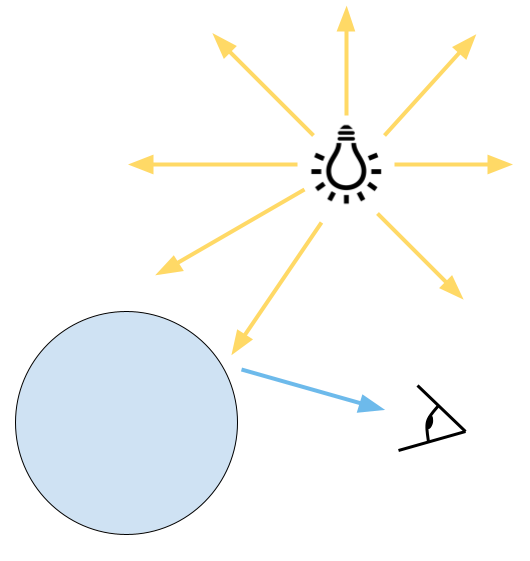
\includegraphics[scale=0.3]{figures/ForwardRT.png}
    \caption{Scene with a single point light and sphere. Note that the viewport captures a limited amount of all light in the scene.}
    \label{fig:forward_rt}
\end{figure}

\noindent
Directly simulating this process is inefficient as only a small fraction of the light produced in the scene will hit the camera. Instead, we can perform the reverse, by casting rays from the camera's viewport and determining how they subsequently interact with the scene and light sources in order to produce an image from the camera's perspective.